\newpage
\section{Image Classification pipeline}

Problem: Semantic Gap (计算机与人看到的完全不一样)

Challenges:
\begin{enumerate}
    \item Viewpoint variation
    \item Illumination
    \item Deformation
    \item Occlusion
    \item Background Clutter
    \item Intraclass variation
\end{enumerate}

An image classifier: 
no obvious way to hard-code the algorithm for recognizing a cat, or other classes. 一个尝试是找角落(有一定的不变性, 但不多)

Data-Driven Approach:
\begin{enumerate}
    \item Collect a dataset of images and labels
    \item Use Machine Learning to train a classifier
    \item Evaluate the classifier on new images
\end{enumerate}
数据和程序是等价的, 数据里包含程序, 使用神经网络拟合这个程序

\subsection{First classifier: Nearest Neighbor}
Memorize all data and labels (记住所有的数据与标签)
Predict the label of the most similar training image(然后预测为最接近记忆的标签)

Example Dataset CIFAR10 
\subsubsection{Distance Metric} to compare images 

L1 distance:
\begin{align*}
    d_1(I_1, I_2)=\sum_p |I_1^p -I_2^p|
\end{align*}

Train $O(1)$, predict $O(N)$. This is bad: we want classifiers that are fast at prediction; slow for training is ok. 

\subsection{K-Nearest Neighbors}
Instead of copying label from nearest neighbor, take \textbf{majority vote} from K closest points. (仍是比较图像, 但选择更多的图像权衡自己的label)

\begin{figure}[!htb]
    \centering
    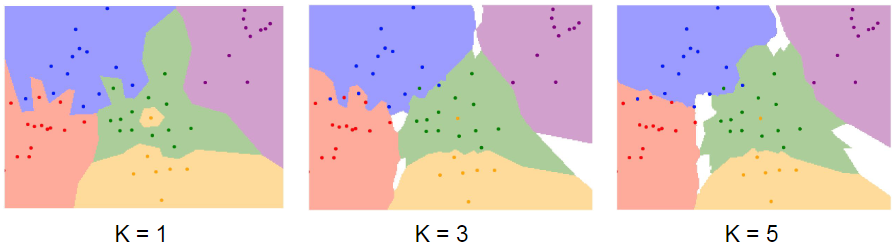
\includegraphics[width=0.42\textwidth]{pic/Lec2/K-nearest}
    \caption{K-nearest (点视为图片高维空间坐标)}
\end{figure}

\subsubsection{Distance Metric}
L2 (Euclidean) distance
\begin{align*}
    d_2(I_1, I_2)=\sqrt{\sum_p(I_1^p-I_2^p)^2}
\end{align*}

\subsubsection{Hyperparameters}
choices about the algorithm that we set rather than learn. Must try them all out and see what works best

Setting Hyperparameters: 
\begin{enumerate}
    \item Choose hyperparameters that work best on the data 过拟合训练集
    \item Split data into train and test, choose hyperparameters that work best on test data 过拟合测试集
    \item Split data into train, val, and test; choose hyperparameters on val and evaluate on test. 在训练集上训练后, 尝试不同超参数跑验证集, 然后选择效果最好的一组超参数作为程序参数. 然后以此跑测试集就是程序最终的表现. (这不是过拟合验证集吗, 感觉这更多只是为了论文的可比较数据, //TODO  但为什么这可比较? 或者说什么是可比较) 
    \item Cross-Validation (Useful for small datasets, but not used too frequently in deep learning) Split data into folds, try each fold as validation and average the results
\end{enumerate}

k-Nearest Neighbor on images never used.
\begin{enumerate}
    \item Very slow at test time
    \item Distance metrics on pixels are not informative
    \item Curse of dimensionality (训练的点需要尽可能覆盖空间, 但这不太可能)
\end{enumerate}

\subsubsection{Summary}
The K-Nearest Neighbors classifier predicts labels based on nearest training examples. 

Choose hyperparameters using the validation set; only run on the test set once at the very end. 

\subsection{Linear Classification}
\subsubsection{Parametric Approach}
\begin{align*}
    f(x, W)=Wx
\end{align*}
$x$ is image, $W$ is parameters of weights. Output is 10 numbers giving class scores. 

\subsubsection{Interpreting a Linear Classifier}

把矩阵中的一行理解为模板在高维空间中的位置, 点积就是估计输入与此行的相似度, 越相近值越大. 偏执独立给出了此类的分数的缩放. 线性分类器只是在学一个模板. 

可视化每一行矩阵, 了解其到底学了什么. 

在高维空间中, 线性分类器是分割不同的坐标点的超平面. \textbf{左下角}的图很关键, 现在我们把图片点视为二维$(x,y)$, 线性分类器就是一系列函数$a_i x+b_iy+c_i$, 其代表了一个平面, 分类结果就是把$(x,y)$输入一系列函数后取最大值的函数$i$作为标签. 
\begin{figure}[!htb]
    \centering
    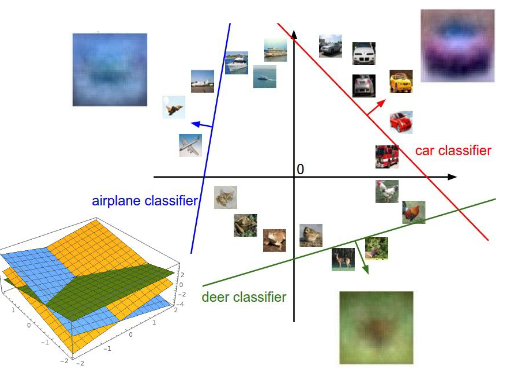
\includegraphics[width=0.309\textwidth]{pic/Lec2/Interpreting a Linear Classifier}
    \caption{Interpreting a Linear Classifier}
\end{figure}

\begin{figure}[!htb]
    \centering
    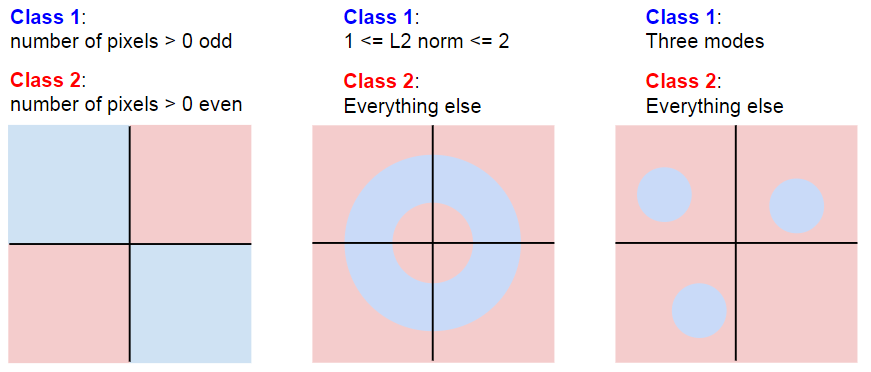
\includegraphics[width=0.42\textwidth]{pic/Lec2/Hard cases for a linear classifier}
    \caption{Hard cases for a linear classifier}
\end{figure}
只有两类的分类器只能划出一条线(两个平面只有一个交线). 最右边表示多模态数据. 